\section*{Introduction}%see https://www.gutenberg.org/files/59883/59883-h/59883-h.htm
Specimen preparation and curation methods are fundamental skills for any entomologist, especially when one needs to prepare and deposit \textit b{vouchers}\citep{vouchersHuber,vouchers1}. This chapter provides guidance on current best practices and the standards used at the Frost Entomological Museum. The taxon-focused chapters in this manual also provide information on best practices (\textit{e.g.}, see Grylloidea, Blattodea, Tipulidae), when they deviate slightly from the general specimen prep approaches described below. Most of this content was adapted from SOP publications by the USDA \citep{USDAmanual,USDAmanual1986}, and the methods described below are by no means a complete accounting of how arthropods are prepared!

\section*{Preparing Hexapoda and related taxa}
Some rules of thumb, to start your journey: 
\begin{enumerate}
    \item If the specimen \textbf{has wings and is longer than 1 cm}, it'll likely need to be pinned (yellow jackets, scarab beetles, butterflies, \textit{etc}.) --- Go to section \ref{pinning}.\\
    \textit{Except} if it's \textbf{a dragonfly or damselfly} (Odonata), it should go into acetone and then into a cellophane envelope --- Go to section \ref{odeprep}\\
    \textit{And except} if it's an \textbf{adult mayfly (Ephemeroptera), stonefly (Plecoptera), or caddisfly (Trichoptera)}, it should go in ethanol --- Go to section \ref{ethanol}
    \item If the specimen \textbf{has wings and is smaller than 1 cm}, it'll likely need to be point-mounted (small wasps, beetles, flies, ants, \textit{etc}.) --- Go to section \ref{pointing}.\\
    \textit{Except} if the specimen is \textbf{covered in scales}, it'll likely need to be double-mounted (small moths, mosquitoes, \textit{etc}.) --- Go to section \ref{doublemount}
    \item If it's \textbf{soft-bodied and relatively large}, you will preserve it in ethanol (spiders, caterpillars, grubs, silverfish) --- Go to section \ref{ethanol}
    \item If it's \textbf{relatively soft-bodied and/or quite small} (springtails, lice, aphids, thrips, fleas), it should be probably be slide-mounted (but putting in ethanol is a good first step) --- Go to section \ref{slides}
\end{enumerate}

\section{Pinning}\label{pinning}
Pinning is the best way to preserve hard-bodied, medium to large pterygotes (\textit{i.e.}, winged insects but not usually Odonata; see below). One should use high quality insect pins, rather than common pins used in sewing and other crafts. Insect pins range in size from 000 (VERY thin and mostly unmanageable) to 7 (very thick and longer than most pins). We recommend sizes 1, 2 (especially), and 3 for general use. The best way to pin an insect is to:
 
\begin{enumerate}
\item Hold the dead insect between your index finger and thumb
\item Pass the pin vertically through the mesonotum (usually), slightly to the right of center (except in Lepidoptera, which gets the pin through the center of the mesonotum), such that it emerges near the right mid coxa.  Pin placement often varies slightly by taxon (see Figure \ref{pinthorax})\index[preps]{Lepidoptera}
\item Slide the pin far enough through the body such that approximately 1 cm of pin is left between the insect and the pin head (Figure \ref{pinplace}); this forms the ``handle'' that allows one to manipulate the specimen
\end{enumerate}

\begin{figure}[ht!]
	\centering
  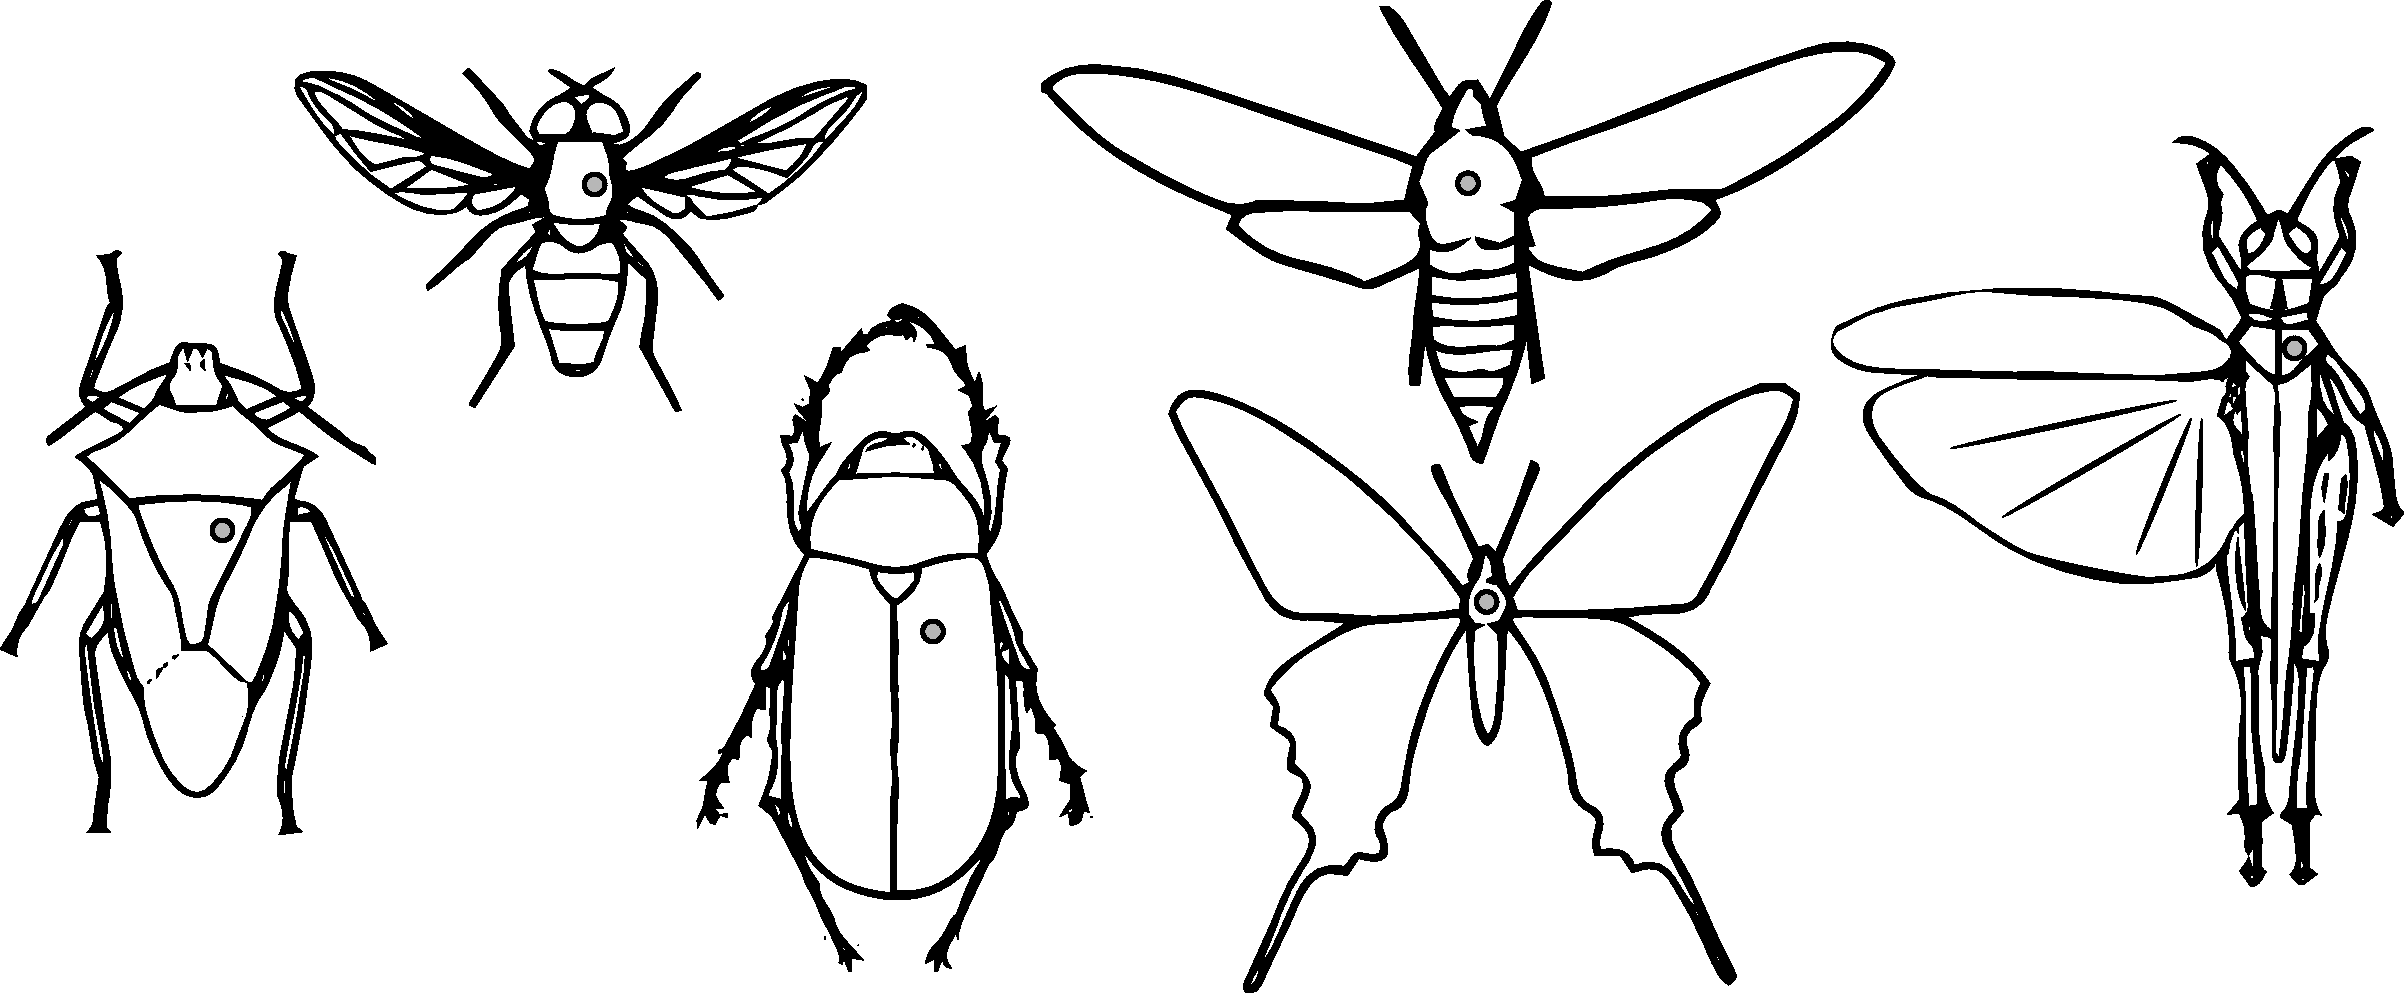
\includegraphics[width=0.9\textwidth]{sections/img/specimenPreps/PinsThorax}
  \caption{Ideal pin placement on different kinds of insects}
  \label{pinthorax}
\end{figure}

\begin{figure}[ht!]
	\centering
  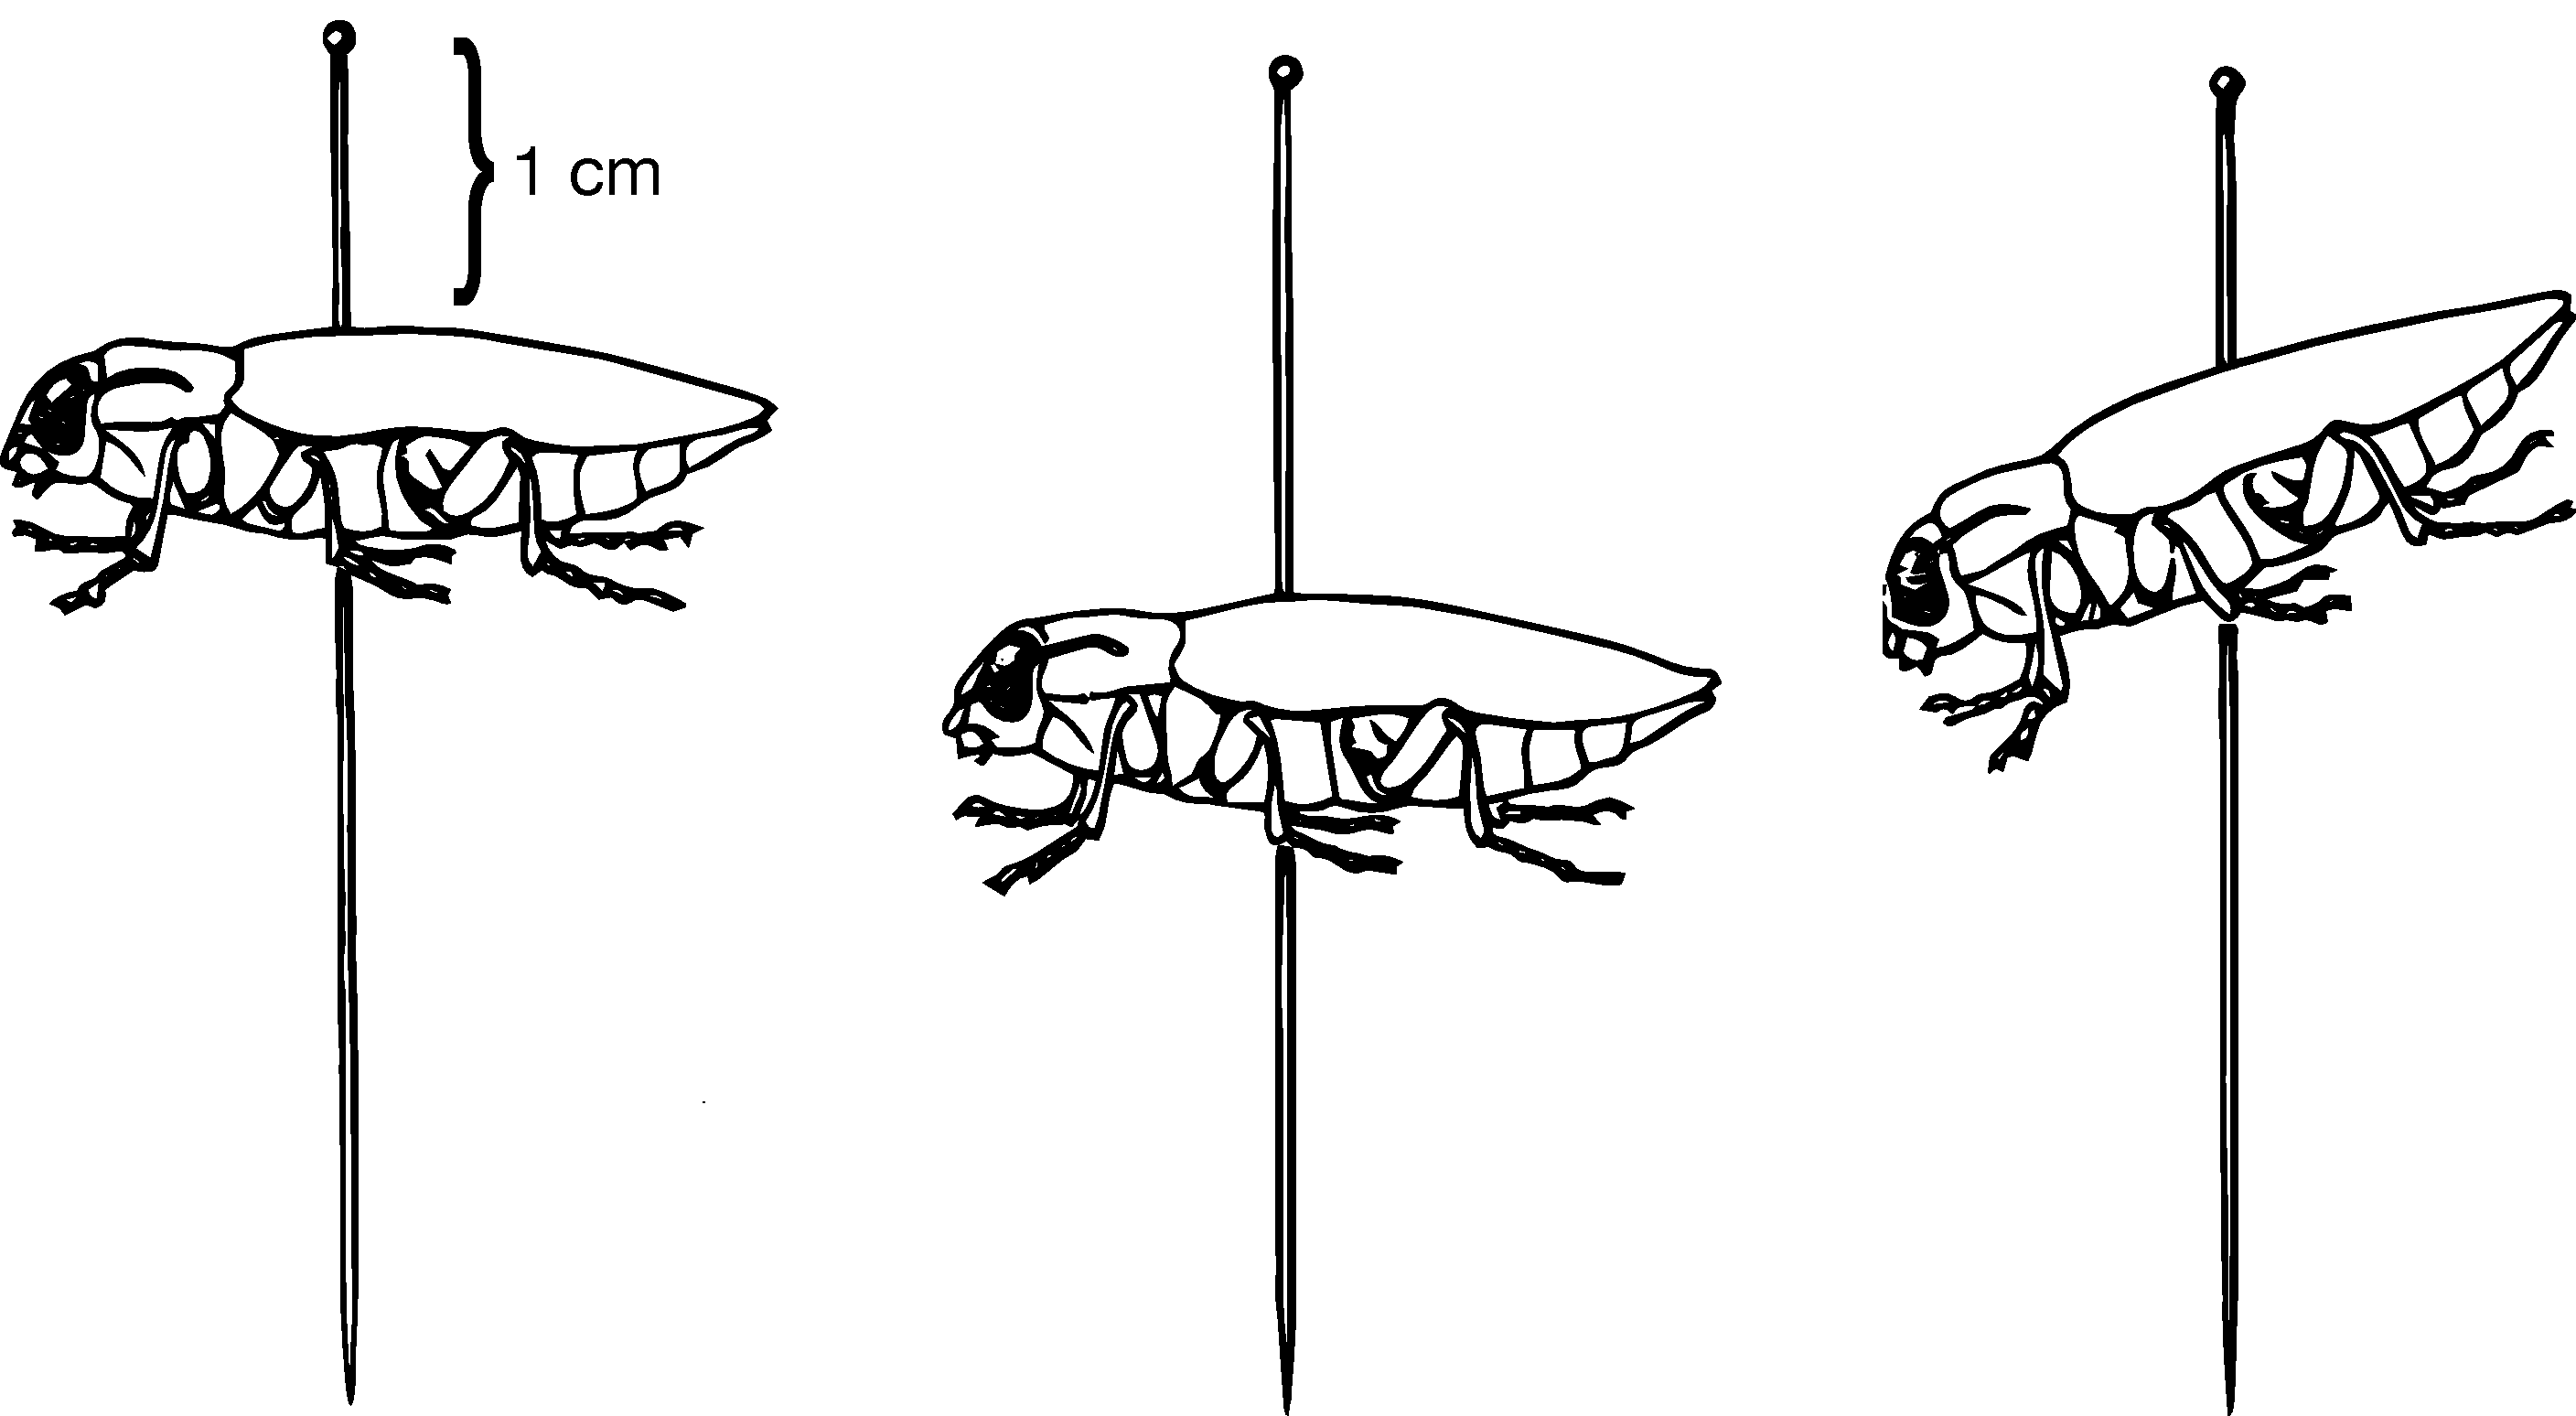
\includegraphics[width=0.52\textwidth]{sections/img/specimenPreps/PinPlacement}
  \caption{Ideal specimen placement on pin (left) and poor placements (middle specimen is too low, right specimen is catawampus) \citep[modified from][Fig. 16]{USDAmanual1986}}
  \label{pinplace}
\end{figure}

\noindent{}Lepidopterans, especially the larger species, need to have their wings spread by using a spreading board (see Figure \ref{lepspread}). Note that Odonata are usually \textit{not} pinned, as they take up too much room with their wings spread. See Section \ref{odeprep}. Also, bees that were collected in ethanol or otherwise look matted can be restored to fluffiness using a process developed by \cite{droegeBee}.

\begin{figure}[ht!]
	\centering
  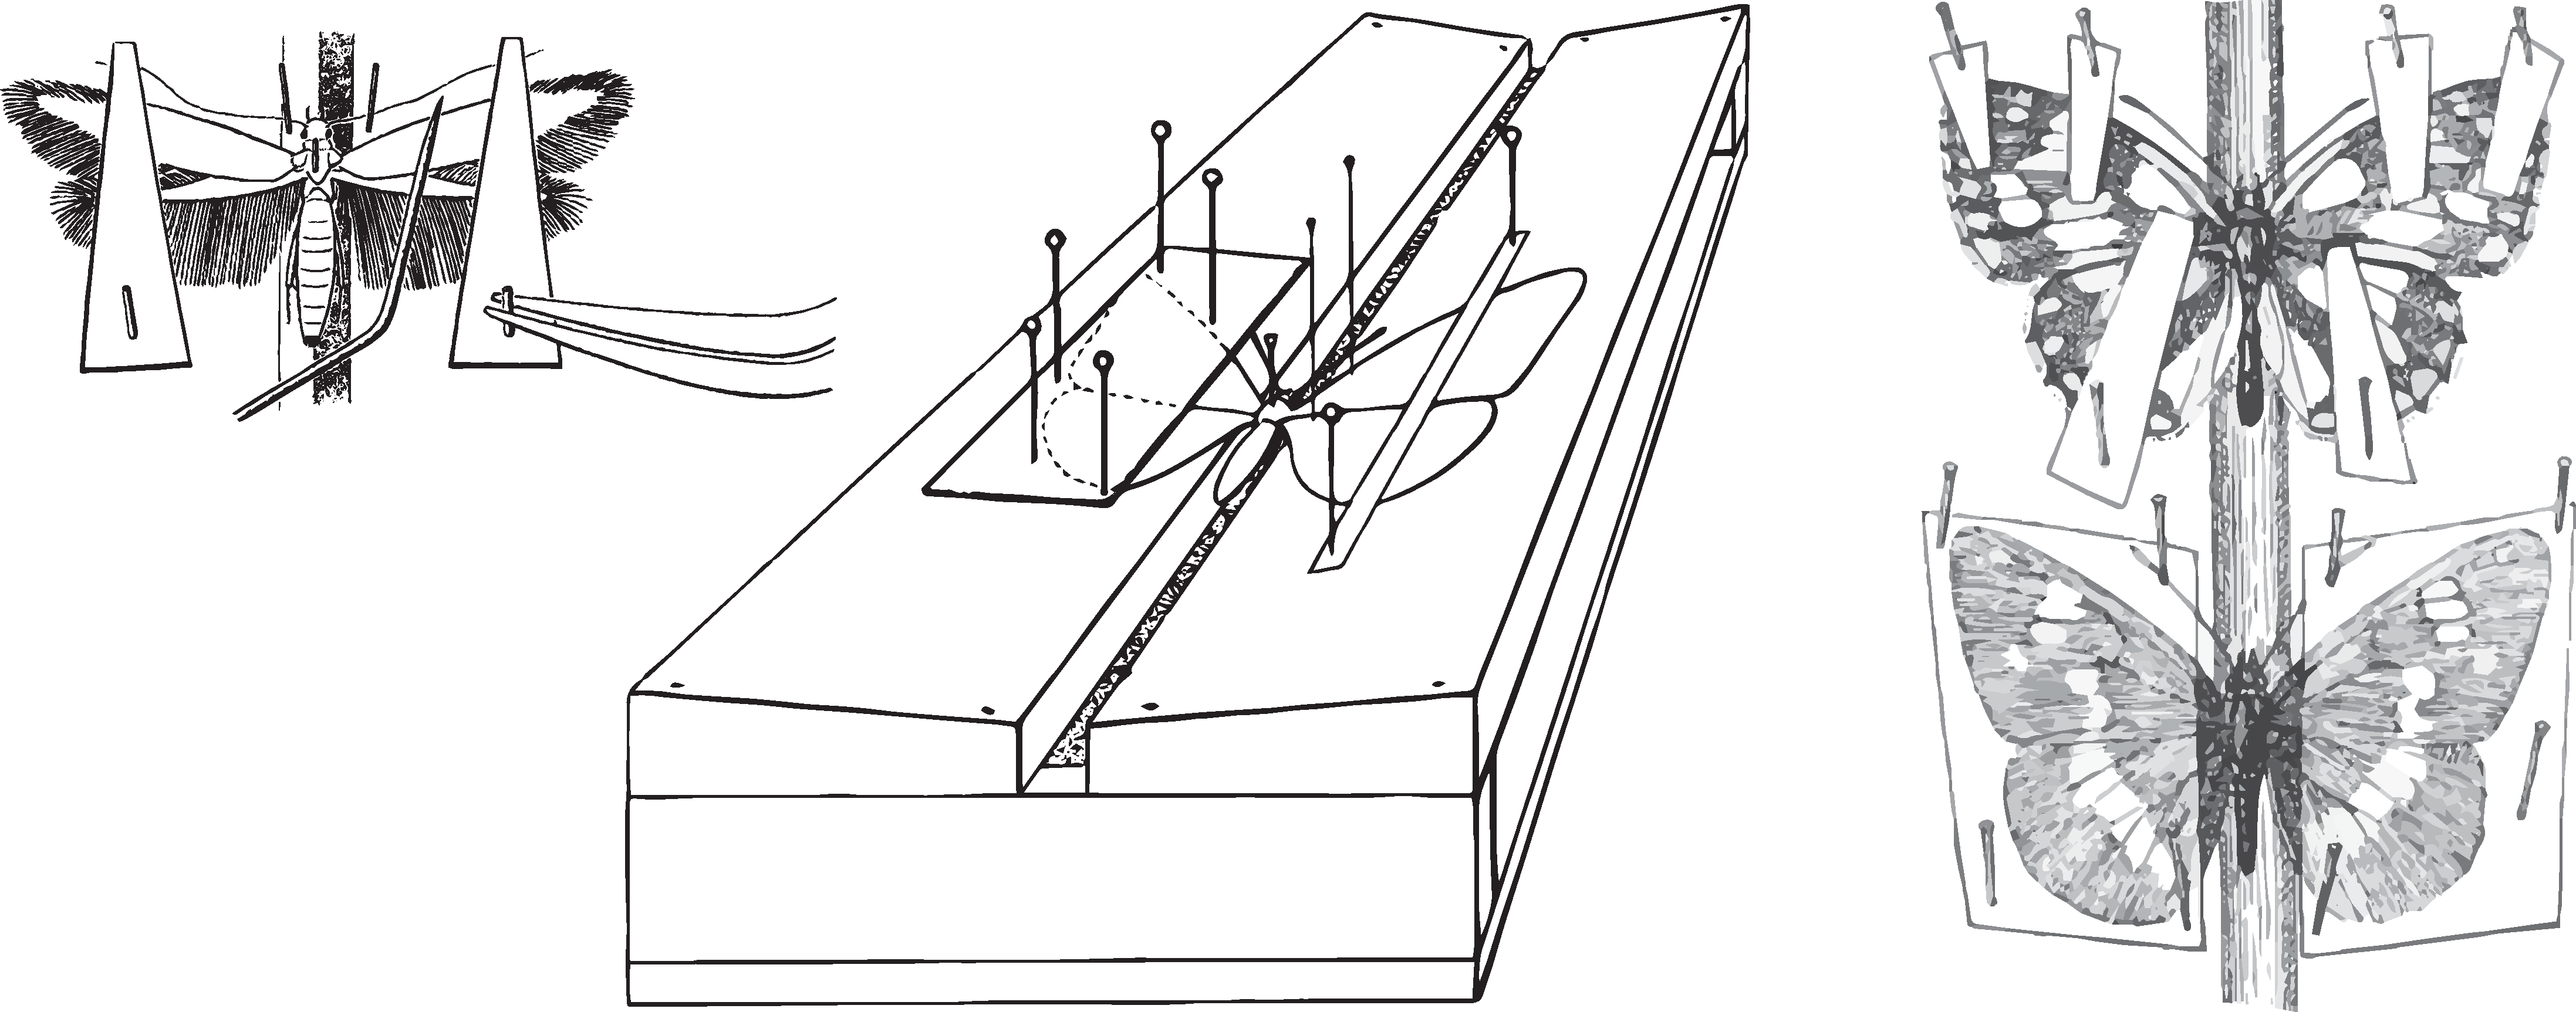
\includegraphics[width=0.85\textwidth]{sections/img/specimenPreps/spreadingLeps.pdf}
  \caption{How to prepare lepidopteran specimens using a spreading board \citep[redrawn from Figs. in][]{bhlitem105840ross,south2022butterflies,landry1994technique}}
  \label{lepspread}
\end{figure}

\section{Point-mounting}\label{pointing}
Smaller insects are usually glued to a triangle (a ``point'') cut or punched from acid-free cardstock or Bristol board (preferred). Place a drop of archival adhesive (\textit{e.g.}, MONO Aqua Liquid Glue), on the tip of a point that has already been pinned. Touch the point tip to the mesosternum of the insect, usually between the fore and mid coxae. The pointed insect should be oriented in a similar position to that of a pinned insect (Figure \ref{fig:points}).

\begin{figure}[ht!]
    \centering
    \begin{subfigure}[ht!]{0.38\textwidth}
        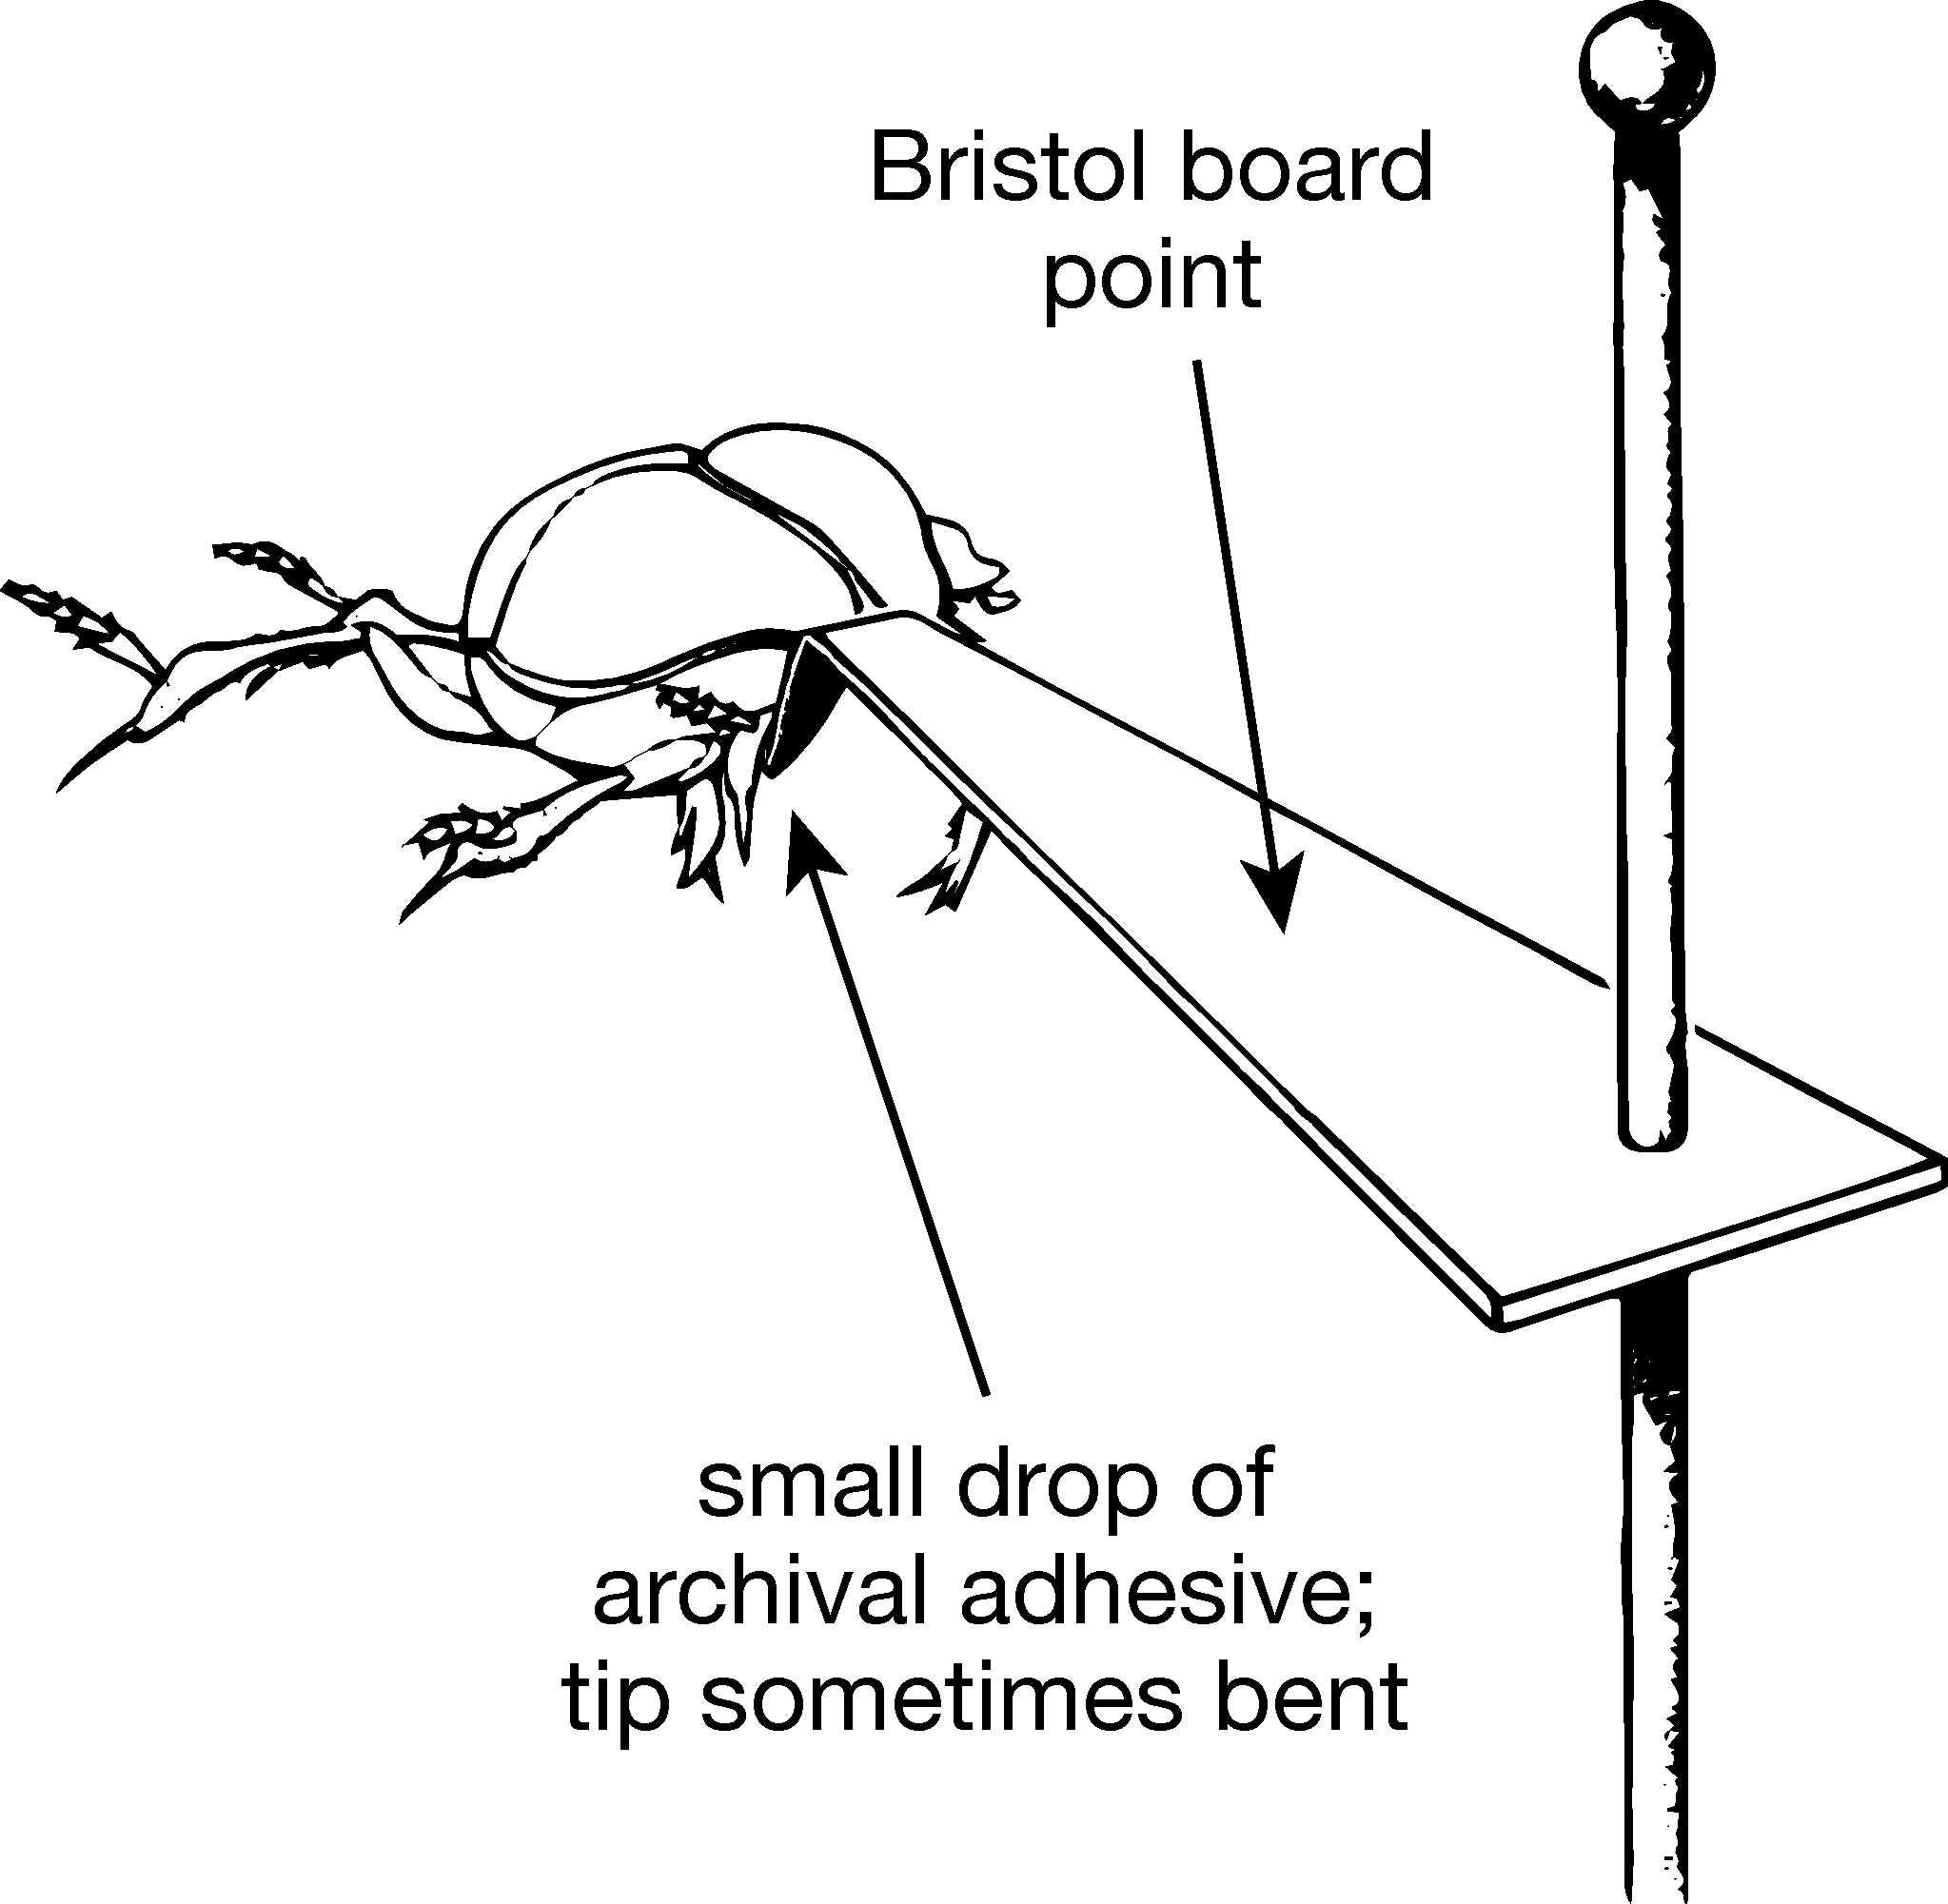
\includegraphics[width=\textwidth]{sections/img/specimenPreps/pointedBeetle}
        \caption{Coleopteran on point \citep[adapted from][Fig. 18C]{USDAmanual1986}}
        \label{fig:beetlepoint}
    \end{subfigure}
    \qquad
    \begin{subfigure}[ht!]{0.31\textwidth}
        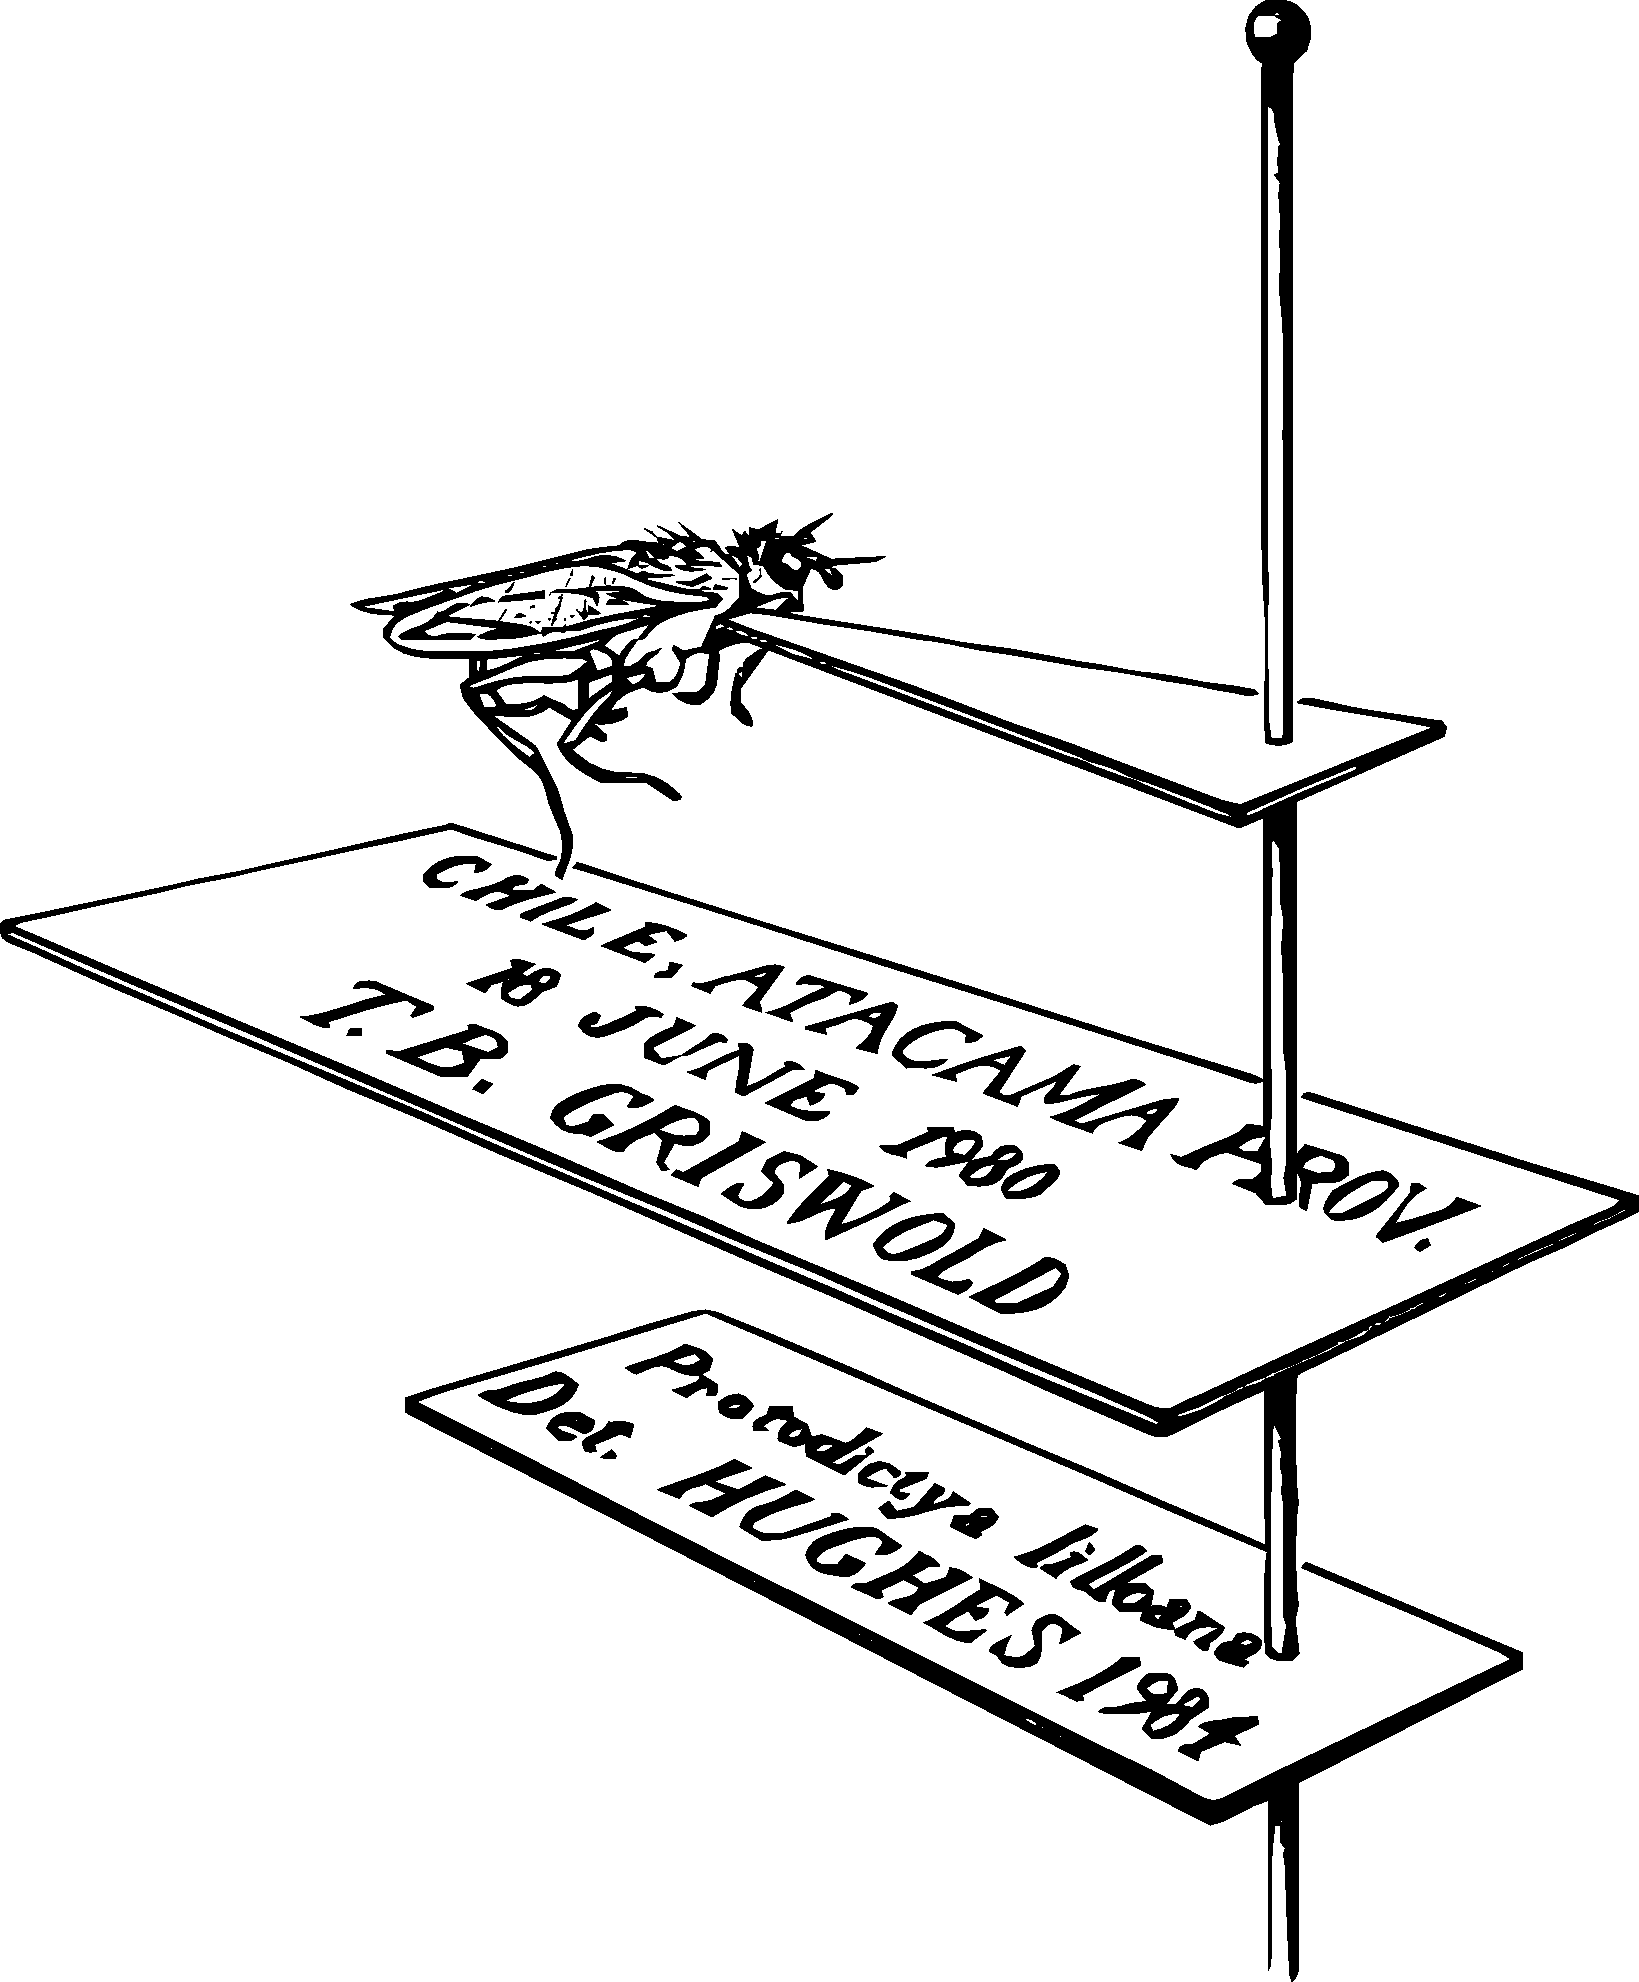
\includegraphics[width=\textwidth]{sections/img/specimenPreps/pointedFly}
        \caption{Dipteran on point \citep[][Fig. 24]{USDAmanual1986}}
        \label{fig:flypoint}
    \end{subfigure}
    \caption{}\label{fig:points}
\end{figure}

\section{Double mounts}\label{doublemount}\index[preps]{Culicidae}
Microlepidopterans and scaly flies (\textit{e.g.}, Culicidae) need to be double-mounted using minuten pins. Essentially this is the same as pinning, except one uses a very small pin (the minuten) to mount the specimen. That mount is then affixed to a normal-sized insect pin via a small piece of foam or silicone (Figure \ref{fig:doublemount}). A more detailed description of this process is provided by \cite{GrinterWebpage}.

\begin{figure}[ht!]
    \centering
    \begin{subfigure}[ht!]{0.32\textwidth}
        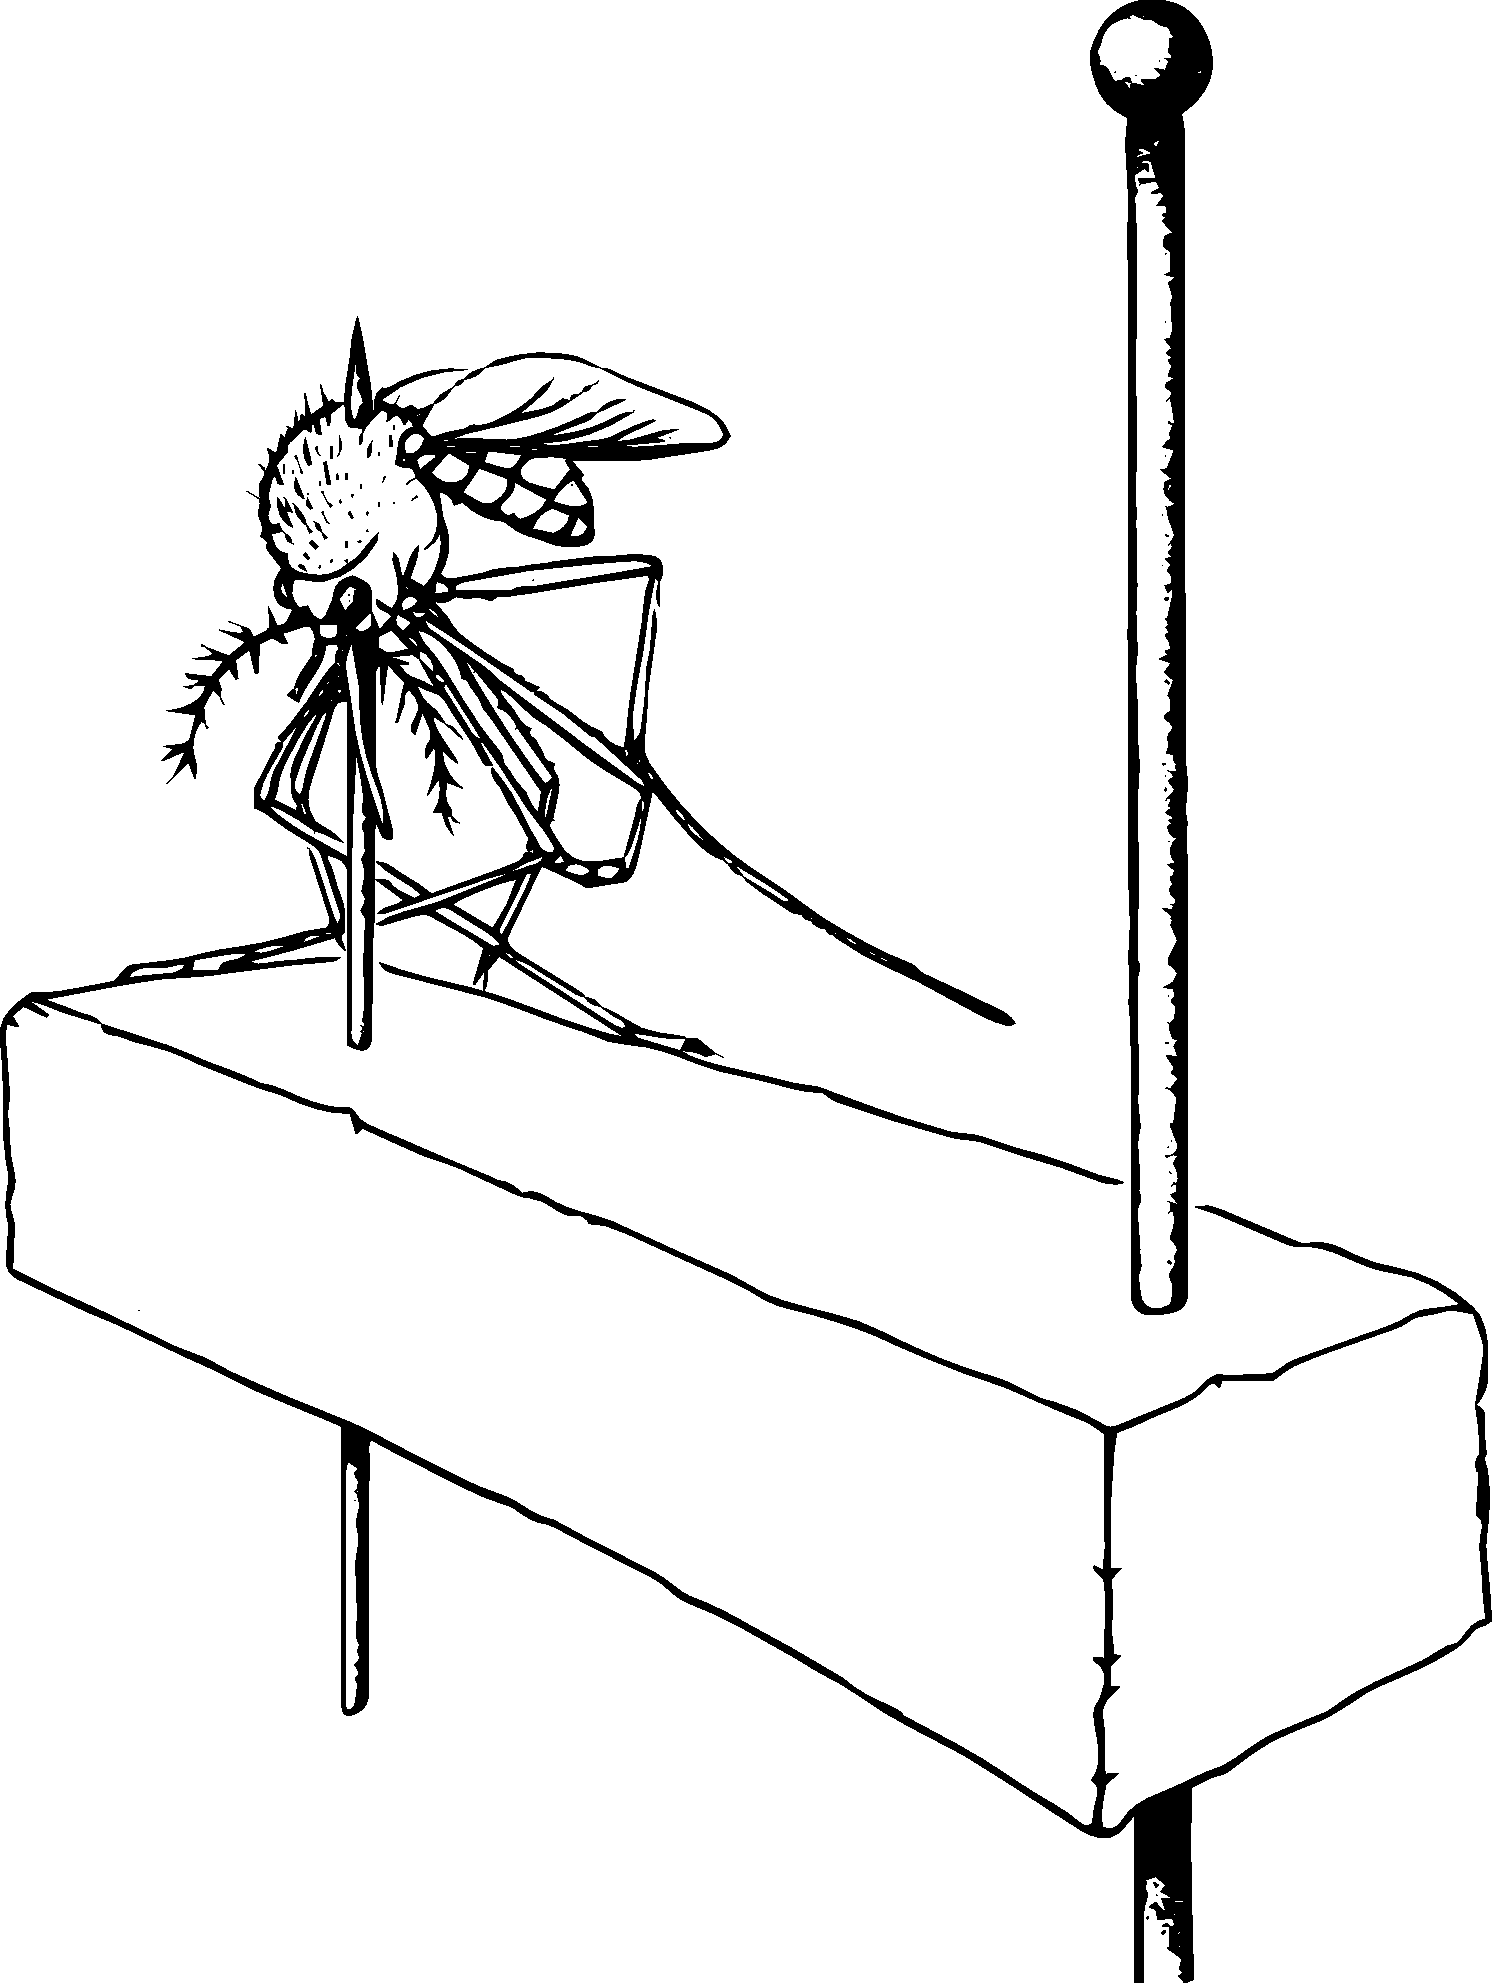
\includegraphics[width=\textwidth]{sections/img/specimenPreps/doublemount}
        \caption{Dipteran on double mount \citep[modified from][Fig. 18A]{USDAmanual1986}}
        \label{fig:flymount}
    \end{subfigure}
    \qquad
    \begin{subfigure}[ht!]{0.36\textwidth}
        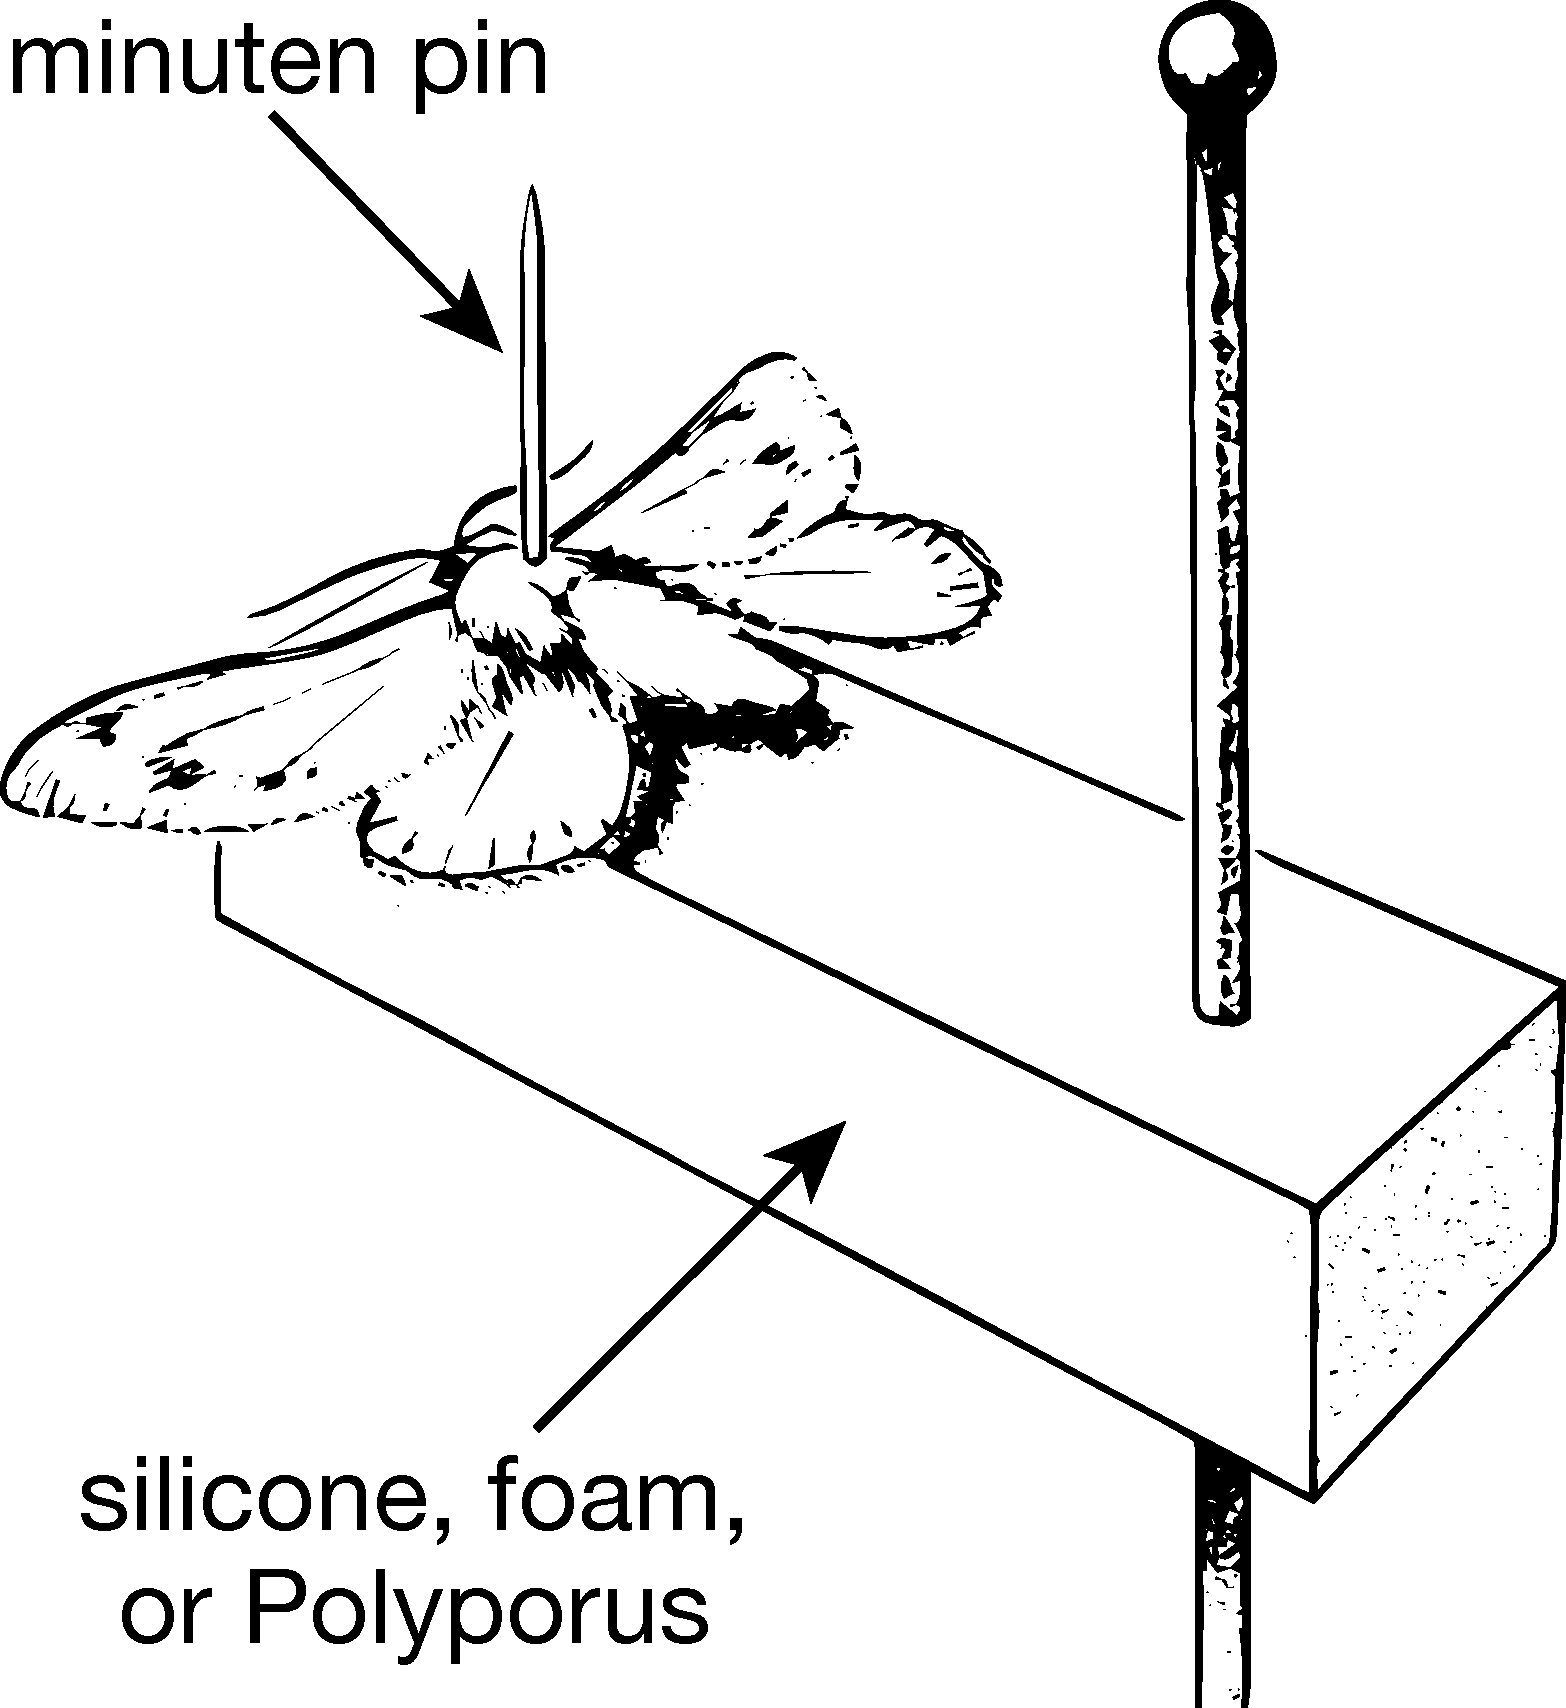
\includegraphics[width=\textwidth]{sections/img/specimenPreps/doublemountMoth}
        \caption{Lepidopteran on double mount \citep[adapted from][Fig. 18D]{USDAmanual1986}; this specimen is arguably too close to the medium but is oriented correctly}
        \label{fig:mothmount}
    \end{subfigure}
    \caption{}\label{fig:doublemount}
\end{figure}

\section{Odonata preparation}\label{odeprep}\index[preps]{Odonata}
Odonata should be kept alive in glassine envelopes, until such time that an acetone bath is available. Allowing them to void the gut while they're alive will result in a better specimen in the end. When ready, follow these steps:
\begin{enumerate}
    \item Using scissors, make a small hole in the glassine envelope by cutting off the corner. This will allow the acetone to drain out later
    \item Submerge the envelope in the acetone, to euthanize the odonate. When it's dead, remove the envelope and adjust the odonate's body, so that the abdomen is straight, the wings are held vertically over the body, and the legs face anteroventrally (see Figure \ref{odeEnvelope})
    \item Place envelope back into the acetone bath and let it sit overnight
    \item Now remove the envelope and let the acetone drain back into the bath. Then let the envelope dry for at least 30 min, preferably in a fume hood or well-ventilated area
    \item The specimen is now ready to be transferred to a cellophane envelope, with its data (collecting event, taxon, \textit{etc}.) printed on an archival 3$\times$5 card
\end{enumerate}
The acetone removes lipids and allows for better overall preservation. For more information see \cite{Tennessen2019}. 

\begin{figure}[ht!]
	\centering
  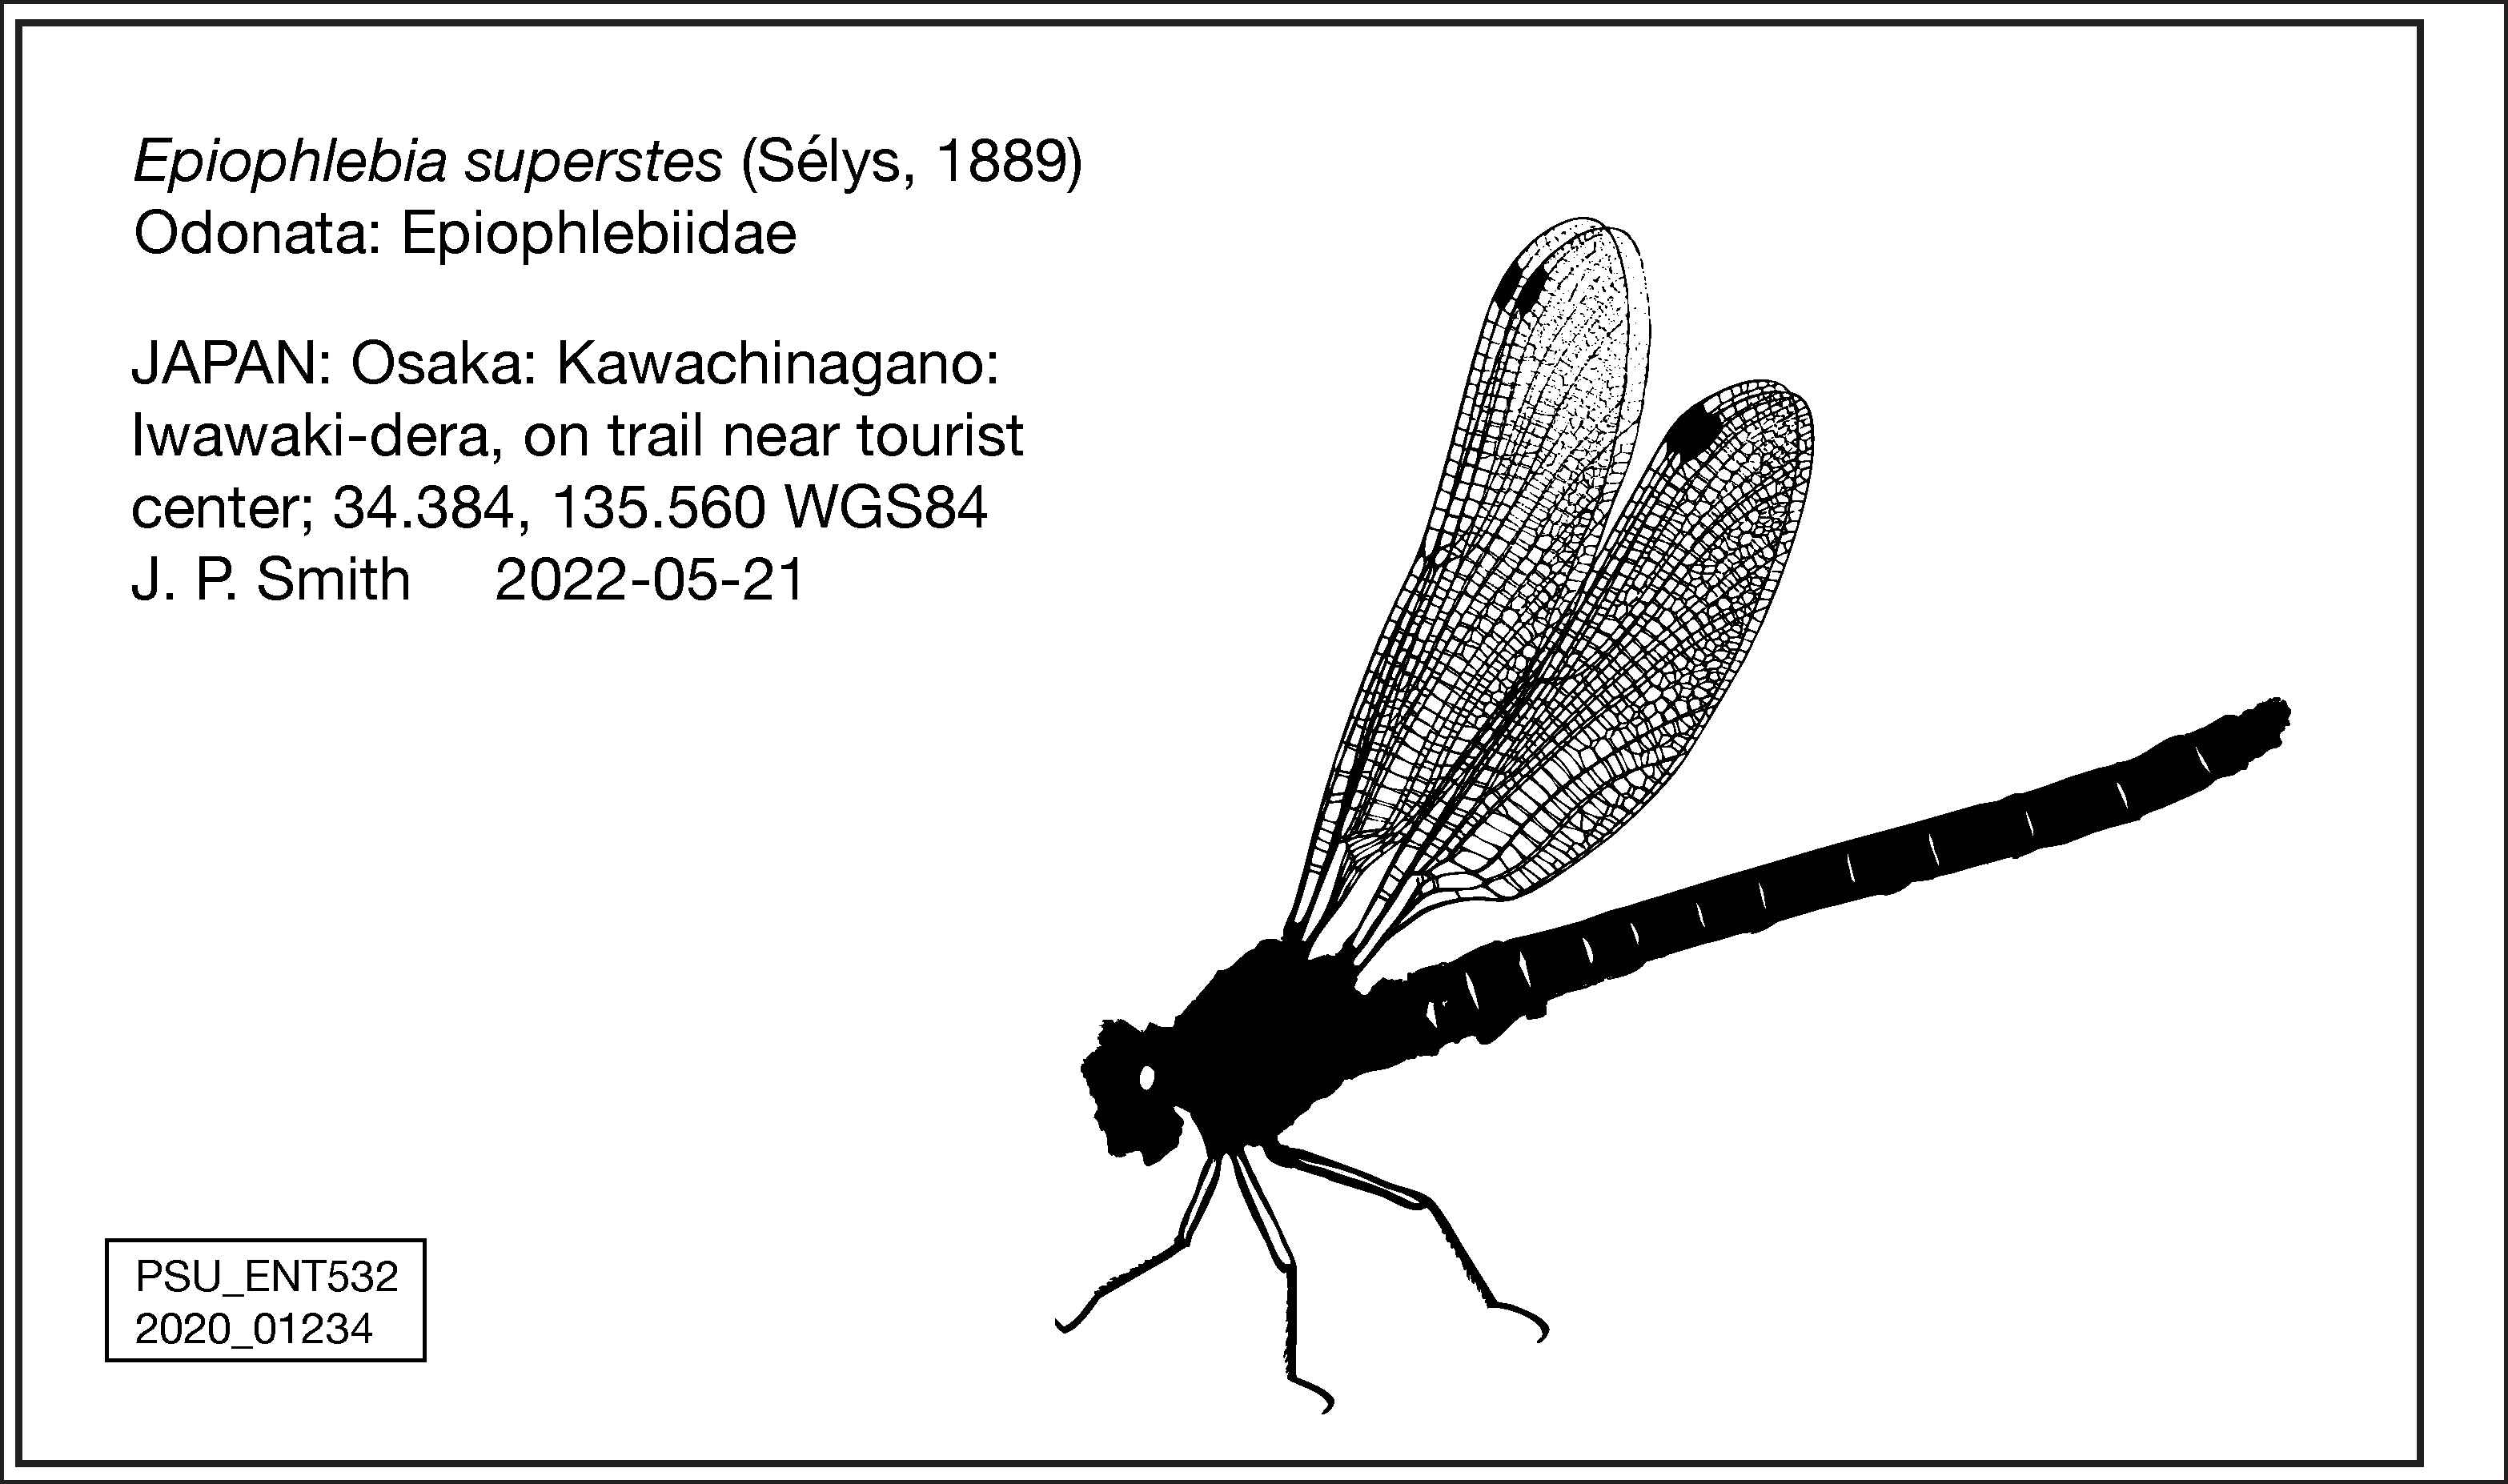
\includegraphics[width=0.8\textwidth]{sections/img/specimenPreps/OdonataEnvelope.pdf}
  \caption{Example of odonate in a cellophane envelope}
  \label{odeEnvelope}
\end{figure}


\section{Dry specimen management}\label{DrySpecimenManagement}
\noindent{}The following guidance should be helpful when preparing and curating dry-mounted insect specimens:
\begin{itemize}
    \item Most taxa are best mounted with the fore legs oriented anteriorly (\textit{i.e.}, pointing forwards) and the middle and hind legs oriented posteriorly (\textit{i.e.}, pointing backwards)
    \item Many insects (e.g., katydids, longhorn beetles, some wasps) have extremely long antennae; try to gently align them with the insect's body during the mounting process and allow them to dry fully before handling. You may need to use pins to brace the appendages while they dry
    \item Mount specimens directly against thick plastic foam, or use extra pins for propping appendages in place while specimens dry; this strategy will prevent legs, antennae, and other structures from hanging down and interfering with subsequent label placement
    \item Once you've placed a pin through an insect, don't try to remount it! A crooked specimen is far better than a specimen with multiple holes through it
    \item Allow specimens to fully dry before putting them into collection boxes; specimens that still have moisture can grow mold which can spread to other specimens in the same area
    \item Never mount a specimen using a damaged or non-archival pin or point
    \item Heavy or large specimens should be ``braced'' by placing pins on multiple sides of the body to prevent them from spinning and damaging adjacent specimens
    \item When organizing specimens in a storage box, leave sufficient room between individual specimens and between specimens and the edges of unit trays to avoid potential collisions. Never cram specimens into small spaces; see Figure \ref{fig:spacing}F for a good distribution of specimens within a single unit tray
    \item If a specimen breaks \textit{do not} try to repair it with adhesive. Consult with a curator on strategies to keep the broken parts associated with the remainder of the specimen and its labels. Gelatin capsules can be used for this purpose. See section on breakage below
\end{itemize}

\noindent{}As you set out to prepare new specimens or handle those in an existing collection, consider these issues:
\begin{itemize}
    \item The health and safety of the specimen is paramount. Handle specimens with extreme care, so as not to damage them or otherwise affect data quality
    \item Specimens should be prepared in a way that maximizes their observation potential while minimizing their footprint in the storage environment
\end{itemize}

\begin{figure}[ht!]
	\centering
  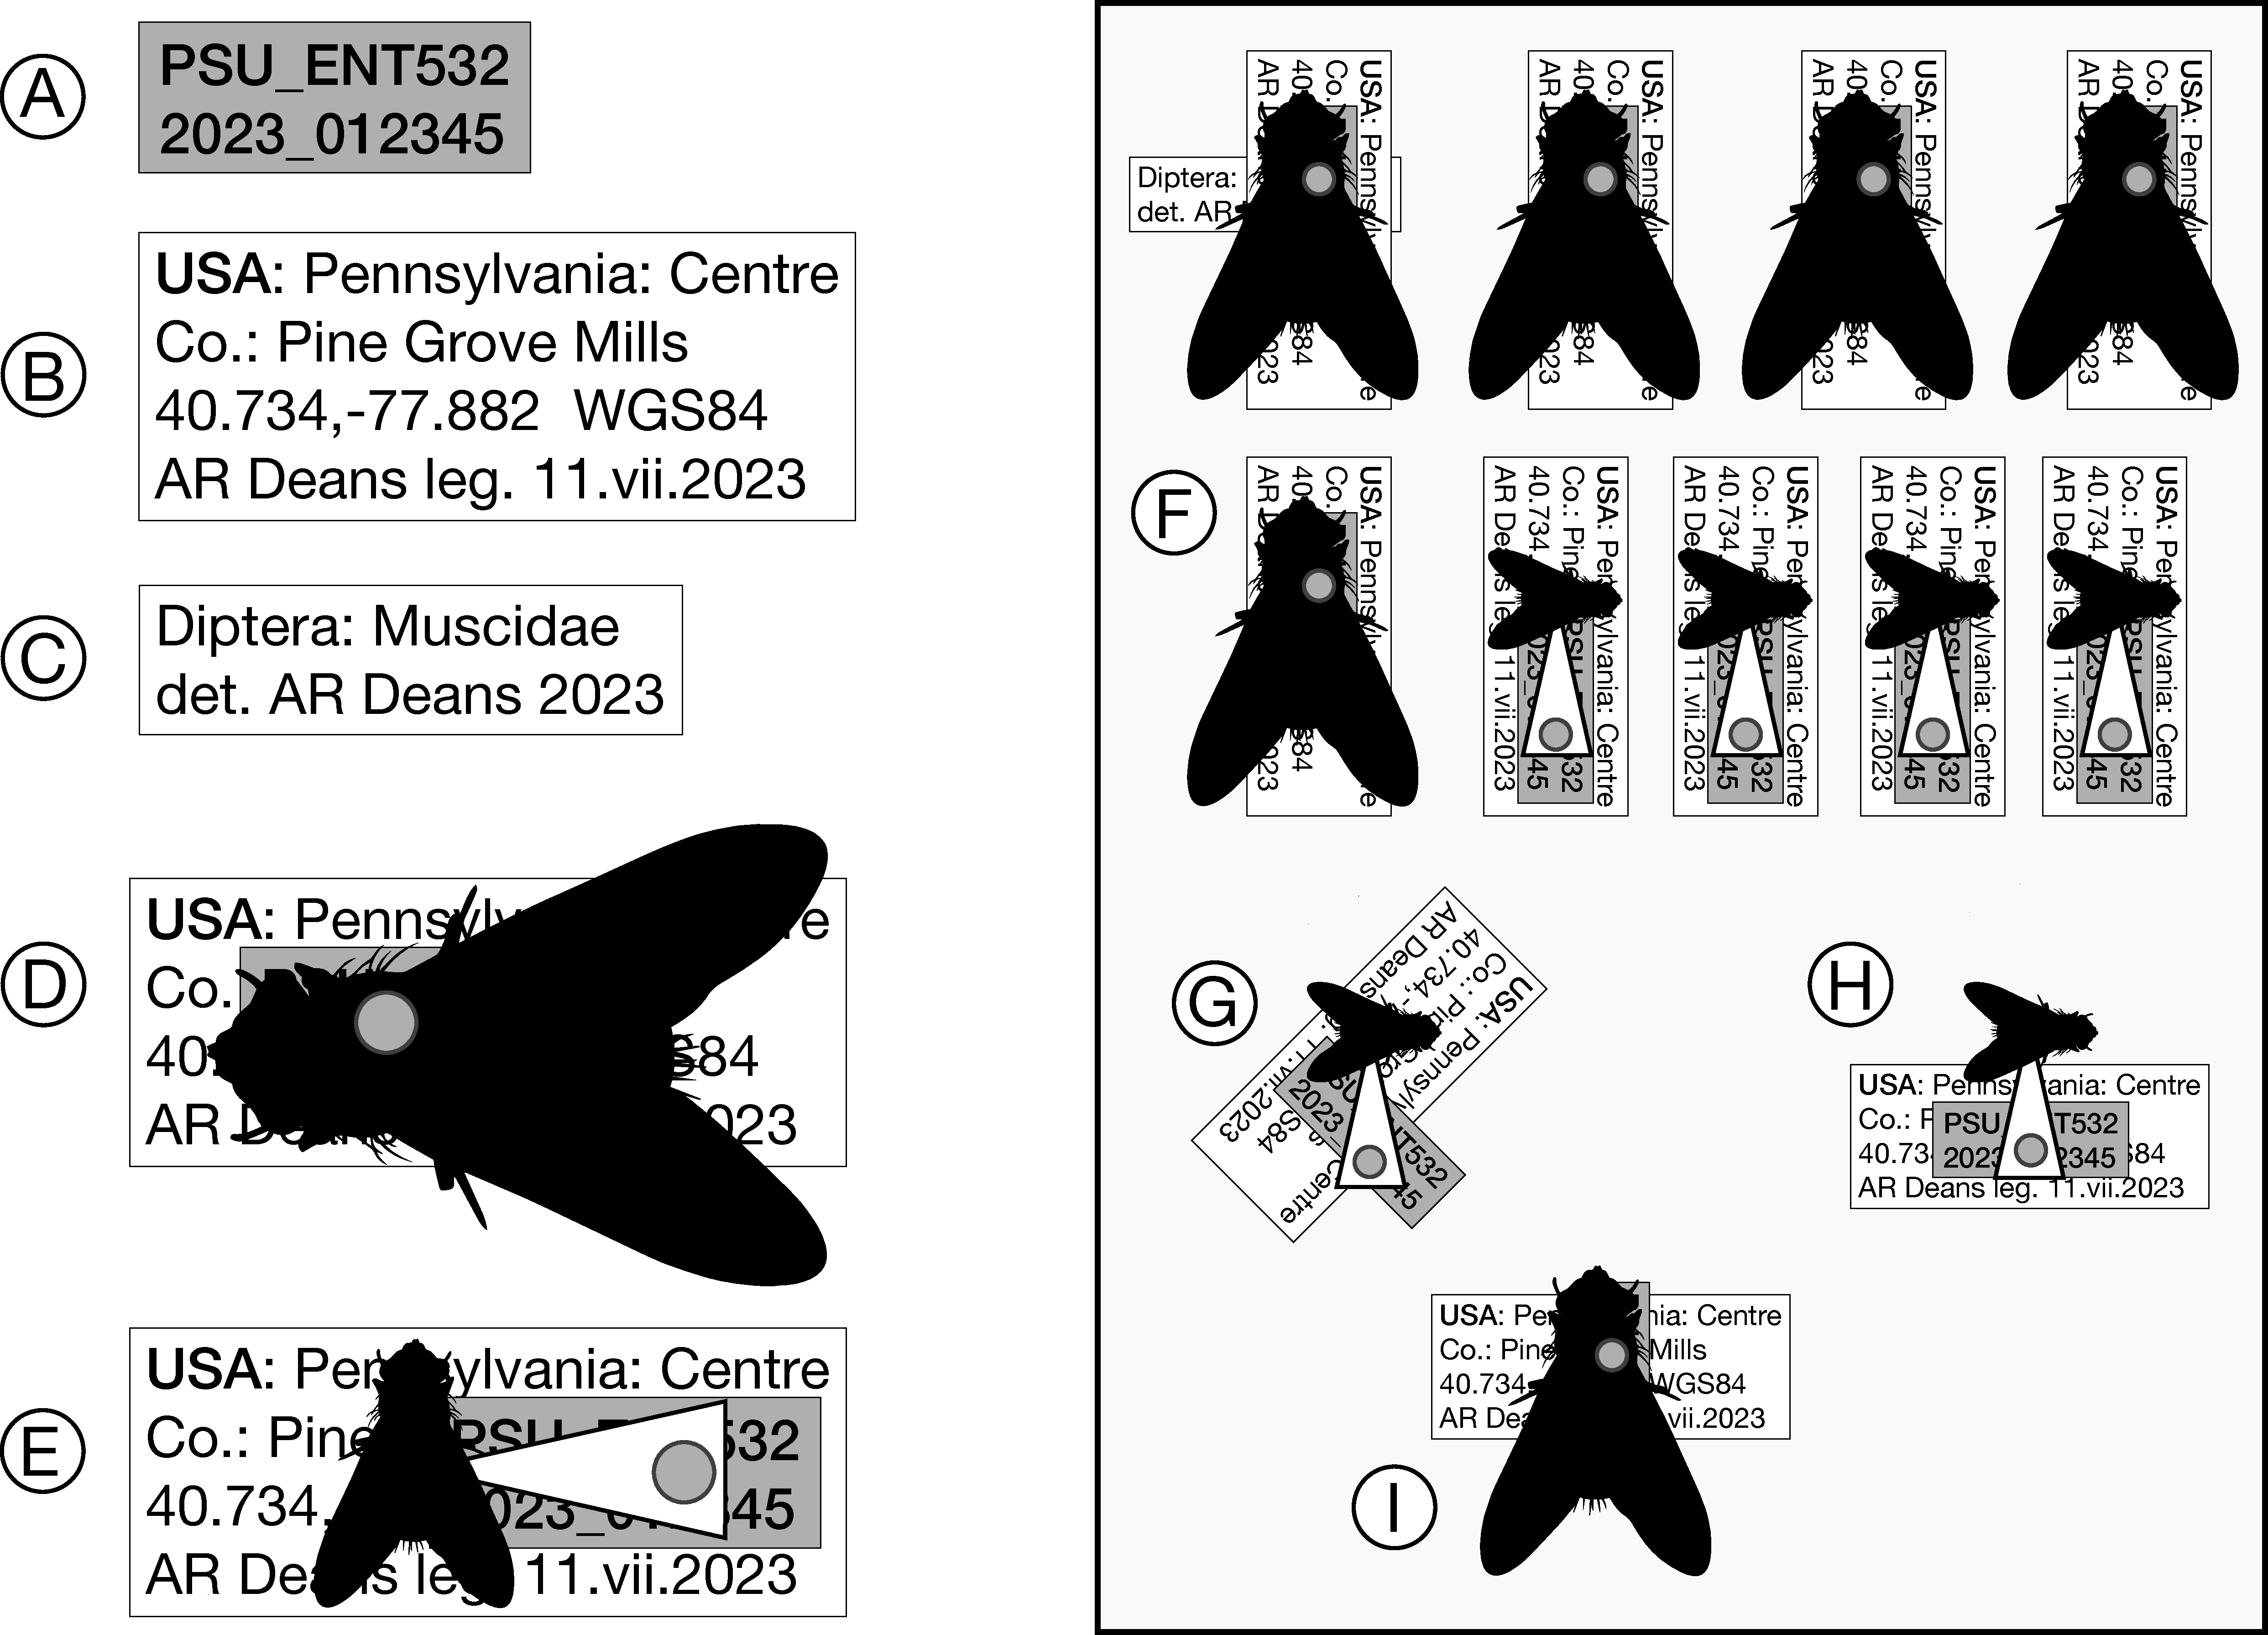
\includegraphics[width=0.82\textwidth]{sections/img/specimenPreps/specimenSpacing}
  \caption{Label orientation and specimen spacing. \textbf{(A)} catalog number, goes directly under specimen; \textbf{(B)} collecting event label, goes under catalog number; \textbf{(C)} determination (``det'') label, goes under collecting event label; \textbf{(D)} orientation of labels on pinned specimen; \textbf{(E)} orientation of labels on point mount; \textbf{(F)} orientation of specimens/labels in unit tray; \textbf{(G)} and \textbf{(H)} incorrect label orientation; \textbf{(I)} incorrect orientation of labels, except on pinned Lepidoptera}
  \label{fig:spacing}
\end{figure}

\subsection{Breakage}
Insects are relatively fragile, especially dried specimens, and breakage is not a rare phenomenon. Broken parts should be treated in a similar fashion to dissected parts, \textit{i.e}, by reassociating them with the primary specimen. For example, if one or more appendages breaks off from a body it/they can be glued to a point or small cut of archival card stock and pinned with the primary specimen. Alternatively one can place them inside a gelatin capsule or genitalia vial that is then pinned with the primary specimen. For Odonata in envelopes, the broken pieces can be placed inside a mini-envelope, cut from a larger envelope, and inserted inside the primary envelope that holds the specimen.

\section{Preservation in ethanol}\label{ethanol}
Soft-bodied hexapods, including spiders and all immature and aquatic insects (except adult Coleoptera), should be preserved in alcohol, rather than being pinned or pointed. Hexapods preserved in \textgreater95\% alcohol are best for DNA extraction, especially if they are kept cold. Unfortunately, high concentrations of alcohol also tend to make specimens fragile, by dehydrating them. Concentrations below 70\% are generally not recommended, as specimens may rot. \\

\noindent{}We use 70--80\% ethanol (with 20--30\% distilled water and sometimes with 1\% glycerin or propylene glycol, to guard against drying out), which works well for nearly any kind of hexapod. Preparation procedure:
\begin{enumerate}
\item Soft-bodied arthropods are best killed in boiling water, which will usually result in a body that is ``spread out'' and partially fixed (like a hard-boiled egg). Once killed, place them inside a shell vial or screw cap vial. There should be one species per vial
\item Insert locality label and identifier label. See label standards below
\item Fill with 70--80\% ethanol mixture
\item If using a shell vial insert cotton wad or polyethylene stopper. Otherwise cover with screw cap. Be sure all air bubbles are removed
\item Place shell vial on cotton pad inside jar. Ideally a jar would contain a single species or several species in a genus. If using a screw cap vial make sure cap is on tight and place into storage box. Make sure jar/box is numbered and labeled with taxon and fill date
\end{enumerate}

\noindent{} Adult Lepidoptera should not (ideally) be preserved in ethanol, as the scales will detach.

\section{Slide mounting}\label{slides}
Slide-mounted preparations are critical for proper diagnosis of certain taxa, especially small insects. The methods are typically intensive and are covered by another SOP document \cite{SlideMounting}.

\section{Specimen labeling}
\subsection{Label order on pins}
Label order should \textit{always be preserved}, as it provides a historical record for that specimen. We typically deal with two kinds of scenarios in the collection:
\begin{itemize}
\item Historical specimens that need identifier labels and/or new determination (det.) labels. In these cases always put the identifier below the last historical label and any new determination labels below the identifier.
\item Recently prepared/labeled specimens that previously had no labels. In these cases put the identifier label on first, then the collecting event, then the determination label.
\end{itemize}
When is it okay to discard a label? Assume \textit{never}. Some labels, however, do not offer any obviously important data---a ripped, non-archival label that simply offers the family name, for example---and may be discarded at your discretion.

\subsection{Catalog number (identifier) label}
Every specimen or lot should have a unique code associated with it, and ideally the string of numbers and letters would be (somewhat) meaningful and globally unique. For the ENT 532 class, the catalog numbers will be printed by the instructors and will look something like this:\\

\hfill\begin{minipage}{\dimexpr\textwidth-1cm}
\begin{labelfontsmall}
\tiny 
\noindent{PSUC\_ENT532\\2024\_1234}\vspace{2mm}

\noindent{PSUC\_ENT532\\2024\_1235}
\end{labelfontsmall}
\xdef\tpd{\the\prevdepth}
\end{minipage}
\normalsize\vspace{2mm}

\noindent{}For specimens to be accessioned into the Frost Museum's research collection, sheets of pre-made identifiers are available. All are prefixed with ``PSUC\_FEM'' and include a data matrix code for scanning. Ideally the data matrix portion of the label should be visible from above. These labels are safe to use in ethanol and other liquid preservatives.

\subsection{Collecting event label}
Collecting event (CE) labels can take many forms, but you generally want to adhere to the following formats:

\begin{enumerate}
\item Labels always begin with the country (sometimes in \textbf{bold} or ALL CAPS) and continue with finer scale details of the locality. One should always include the latitude and longitude---using decimal based degrees is preferred over minutes and/or seconds, as they are easier to database.
\item The date should be formatted such that the month is in lowercase Roman numerals (\textit{e.g.}, October would be ``x''): 12.x.2022 or 11--12.x.2022 or 11.x--12.xi.2022. You could also use the ISO 8601 standard format: YYYY-MM-DD.
\item The collector's name(s) should also be included, as should the collecting method. Common abbreviations include: MT = Malaise trap, YPT = yellow pan trap, FIT = flight intercept trap, SS = screen sweep. Collectors' names are sometimes followed by ``leg.'', which is short for the Latin \textit{lego}, to gather or collect.
\item A sans-serif font makes the label more readable when the size gets small. Most people use 4 pt for the font size. The finished label should be informative, with a minimal amount of abbreviations, but also reasonably small in size. The information should also be presented in a symmetrical label that minimizes white space:\\

\begin{labelfontsmall}
\tiny 
\noindent{\textbf{US}: Pennsylvania: Centre Co.: \\ Pine Grove Mills, 40.730, \\ -77.884, $\pm$ 500m 15.iv.2024 \\ leg. A.R. Deans, sifted litter}
\end{labelfontsmall}
\normalsize

\item Labels that seem to be excessively large can be cut into two labels. Specimens are prone to multiple labeling from future studies (voucher label, determination label, accession numbers, barcodes, \textit{etc.}); it's desirable to keep the label number to a minimum.
\item Use cotton rag, acid free cardstock or similar archival paper for printing labels.
\end{enumerate}

\subsection{Determination Labels}
Determination (``det'') labels can also vary in their appearance, but it's important that they include the taxon name(s), including the author if it's a species-level determination, the name of the determiner, and the year (or date) the determination was made. Det labels for fluid preserved specimens should be in a slightly larger font and more elongate (see Section \ref{fluidspecimen}).\\

\hfill\begin{minipage}{\dimexpr\textwidth-1cm}
\begin{labelfontsmall}
\tiny 
\noindent{\textit{Amphibolips confluenta}\\(Harris, 1841)\\ Hymenoptera: Cynipidae\\ det. A.R. Deans 2024}
\end{labelfontsmall}
\xdef\tpd{\the\prevdepth}
\end{minipage}
\normalsize\vspace{2mm}

\subsection{Labels for fluid-preserved Specimens}\label{fluidspecimen}
Labels for fluid-preserved specimens are similar in design, but one should make the words slightly larger (maybe 6 pt font) and more elongate:\\

\hfill\begin{minipage}{\dimexpr\textwidth-1cm}
\begin{labelfontsmall}
\scriptsize 
\noindent{USA: PA: Centre County: Pine Grove Mills\\ Slab Cabin Run, 40.730, -77.884, $\pm$ 250m \\hand collected off rocks, 15.iv.2024 A.R. Deans}
\end{labelfontsmall}
\xdef\tpd{\the\prevdepth}
\end{minipage}
\normalsize\vspace{5mm}

\noindent{}Small labels act almost like blades and can damage wet-preserved specimens as the vial gets moved around. Longer labels can be wrapped around the inside of the vial in a ring-like manner, or they can fill the vial longitudinally.

%\indexprologue{Here you'll find pages that mention taxon-specific specimen prep recommendations.}
%\printindex[preps] % Output the 'preps' index